% Author: David Sanchez-Jacome

\chapter{Applications using FPPGAs}\label{chap:applications_using_fppgas} % (fold)

The emergence of the field programmable photonic gate array (FPPGA) platform, presented in the prior chapter, powered by a high-level software layer unlocks the door to a wide set of applications.
The Python API layer developed during this thesis enables the users of the platform to synthesize several types of circuits in the mesh where the PUCs can either be configured in cross, bar or tunable coupler states.
We recall that since the PUCs have two drivable arms their coupling factor and cross-phase can be set independently (as covered in Section~\ref{sec:software_stack}), allowing us to expand the flexibility of the configured circuits.
In this chapter we present a set of applications demonstrated on the first-generation Smartlight platform by our team and in collaboration with other research centers around the world.
The chapter puts emphasis on presenting the Python code used to configure and measure these circuits, enabling interested readers to reproduce them using either the hardware platform or the system simulator.

\section{Interconnects}\label{sec:interconnects} % (fold)

\begin{lstlisting}[caption={Implementation of manual and automatic interconnects using the first-generation Smartlight API}, label=lst:ch3-interconnects]
	# Manual configuration
	puc_info = [
		(0, "x"),
		(6, "x"),
		(10, "x"),
		(16, "="),
		(20, "x"),
		(25, "x"),
		(28, "="),
	]
	smart.interconnect(puc_info)
	# Automatic configuration
	PUCs_configuration = smart.interconnect_auto(input_port=0, output_port=6)
	\end{lstlisting}

Reconfigurable optical interconnects are of great interest in optical networks as they enable flexible connections of terabit data rates with high-performance operation \cite{khani_sip-ml_2021}.
These interconnects demand reduced latency and energy efficiency between input and output (I/O) ports, and therefore minimal insertion loss and shortest distance is highly desired.
These circuits are the simplest and can be implemented by manually setting the PUCs to cross and bar states.
This can be done by passing the API a dictionary-like structure specifying the individual states of each PUC.
Additionally, the graph layer presented in Section~\ref{sub:graph_layer} provides an interconnect algorithm based on Dijkstra \cite{foead_systematic_2021,bierlaire_optimization_2015}, which can automatically provide an optimum path configuration.
This automatic implementation can also provide self-healing capabilities to allocate alternative optical paths with lower insertion loss when needed.
The manual and automatic code implementations are presented in Listing~\ref{lst:ch3-interconnects}.

\begin{figure}[h!]
	\begin{center}
		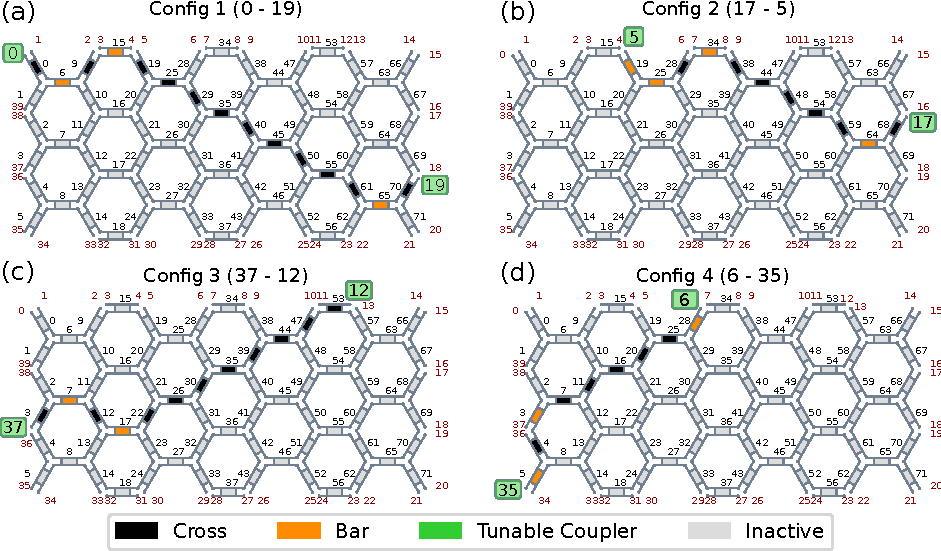
\includegraphics{figures/ch3-interconnects.pdf}
	\end{center}
	\caption{Optical interconnect experiment.
		Programmable path configurations considering different input ports.
	}\label{fig:ch3-interconnects}
\end{figure}

\begin{figure}[t]
	\begin{center}
		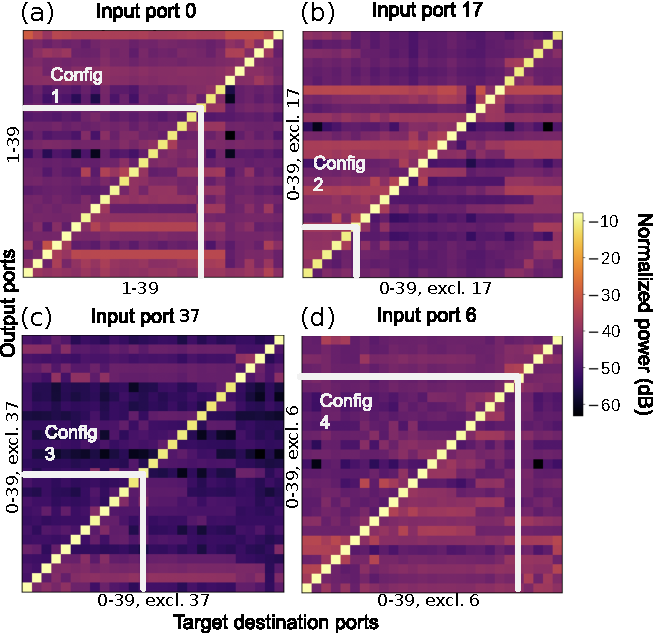
\includegraphics{figures/ch3-inter_power_meter.pdf}
	\end{center}
	\caption{Optical interconnect experiment.
		Colormap of the optical power measured at output ports for different interconnect configurations normalized to the laser input power (5~dBm).
		The white lines indicate the configuration shown in the schematic of the programmable processor.
		The HPB ports [22-33] are not considered as they are neither routed to a PD nor exit the PIC.
	}\label{fig:ch3-inter_power_meter}
\end{figure}

The results of the optical interconnect experiments at a central wavelength of 1550 nm and the processor configurations are shown in Figure~\ref{fig:ch3-interconnects}.
Ports 0, 17, 37 and 6 are used as input ports, and up to 27 interconnects to other available output ports are programmed as the HPB ports [22-33] can't be used as output ports since they are neither routed to a PD nor exit the PIC.
As it can be seen in Figure~\ref{fig:ch3-inter_power_meter}, all the paths are configured successfully, showing diagonal lines in the colormap, each one corresponding to a given interconnect.
The power of the measured output is normalized to the input power of the laser (5 dBm).
The insertion loss at each target port is between 7.7 dB and 10.5 dB, depending on the number of PUCs used to configure the path.
In the experiment, the longest interconnect path consists of 15 PUCs, while the shortest is only 2 PUCs which produces a certain power imbalance between outputs related directly to the losses per PUC (\(\approx\)0.46 dB).
Furthermore, optical power is also measured at the rest of the non-targeted output ports, with an average leakage of -30 dB.
The algorithm allows the simultaneous identification of up to 400 possible paths with an average time of about 0.4 microseconds per path.
% section Interconnects (end)

\section{Beamsplitters}\label{sec:beam_splitters} % (fold)

\begin{figure}
	\begin{center}
		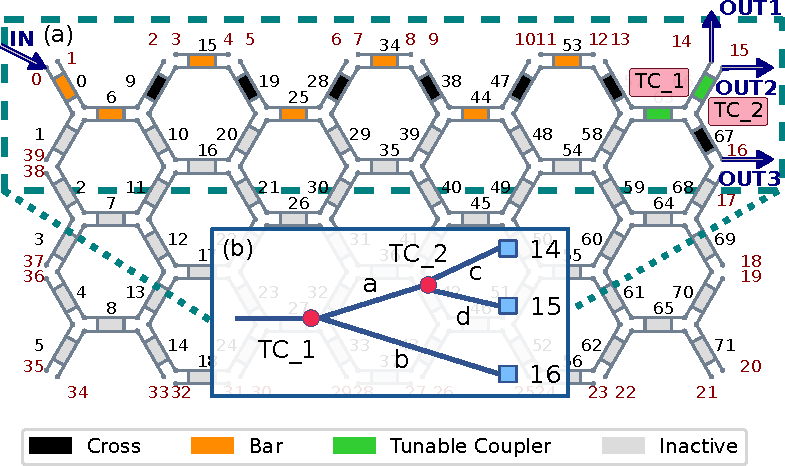
\includegraphics{figures/ch3-splitter.pdf}
	\end{center}
	\caption{Optical beam splitting demonstration: The first-generation Smartlight programmable processor synthesizing a 1x3 splitter configuration.
		The inset shows the detailed graph.
	}\label{fig:ch3-splitter}
\end{figure}

Optical beam splitting allows for a single optical signal to be efficiently distributed across multiple receiving nodes or devices simultaneously.
This is particularly advantageous in scenarios where the same data needs to be delivered to several destinations within a data center cluster, simultaneously.
This functionality is currently not available in the physical layer of most networks.
So, if deployed under the right software stack support it has the potential to open the door to new, cost-efficient and disruptive applications.
One added advantage brought in by PIP is the software-defined control of the splitting ratio across the outgoing signals powered by the fine-tuning of driving phases applied to the PUCs.
As a consequence of this, the operator can then control how much power is allocated to different receiving nodes in a dynamic manner.

Beamsplitter circuits can be implemented manually on the first-generation Smartlight platform similarly to the interconnects presented in the previous section.
In this case however, the state of some PUCs can be set to a floating-point value corresponding to the splitting factors required by the circuit.
A simple example of a 1-by-3 network is demonstrated in Figure~\ref{fig:ch3-splitter}.
The graph representation of the beamsplitter network is useful when determining how the splitting circuit can be mapped on the hexagonal mesh as presented in Fig.~\ref{fig:ch3-splitter}.
In Listing~\ref{lst:ch3-splitter} we define such beamsplitter which uses 0 as input port and ports 14, 15 and 16 as outputs.
The optical splitting happens in PUCs 63 and 66 where the coupling factor is set to 1/3 and 2/3, respectively.
This splits the optical power equally among the three outputs.
The coupling factors of the other PUCs take the value '=' or 'x', which corresponds to bar state (k = 0) or cross state (k = 1).

Additionally, in this work, we have designed an auto-beamsplitter algorithm that can accommodate any number of desired outputs from a given input.
It determines the optimum path to each output, and efficiently autoconfigures the splitting PUCs with a ratio that ensures every output port receives the same power, for a traditional beamsplitter operation, or the specified power ratio, under custom operation \cite{xie_software-defined_2024}.
To achieve this, the auto-beamsplitter algorithm can be translated into a single-source shortest path problem represented by a directed acyclic graph (directed tree) \cite{perez-lopez_programmable_2018}.
As observed in Listing~\ref{lst:ch3-splitter}, the auto-beamsplitter allows the user to define a beamsplitter from the given input and outputs ports, and this functionality will find the specific PUCs to be used and define their coupling factors.
The optimal path will be selected based on the FOM that we defined in Section~\ref{sub:graph_layer}.

\begin{lstlisting}[caption={Implementation of manual and automatic beamsplitters using the first-generation Smartlight API}, label=lst:ch3-splitter]
# Manual configuration
puc_info = [
    (0, "x"), (6, "="), (9, "x"), (15, "="), (19, "x"), (25, "="),
    (28, "x"), (34, "="), (38, "x"), (44, "="), (47, "x"),
    (53, "="), (57, "x"), (63, 1/3), (66, 2/3), (67, "x"),
]
smart.beam_splitter(puc_info)
# Automatic configuration
pucs_configuration = smart.beam_splitter_auto(input_port=0, output_ports= [14,15,16]) 
\end{lstlisting}

When light is divided at a TC it will traverse two different paths, defined here as cross and bar paths, until it reaches the output ports.
The inherent insertion loss difference between these paths will cause an undesired power imbalance at the outputs, i.e., the power ratio between the outputs will not be as intended.
Therefore, it is vital to account for the insertion losses in both paths (cross and bar) coming out of a TC and compensate them to achieve the targeted power distribution, see Eq.~\eqref{eq:ch3-k_nonideal}:

\begin{equation}
	k = \frac{k_T}{(1 - k_T) \cdot 10^{\frac{IL_b - IL_c}{10}} + k_T}
	\label{eq:ch3-k_nonideal}
\end{equation}

where \(k_T\) is the ideal splitting ratio of the tunable coupler PUC, and \(IL_b\) and \(IL_c\) are the bar path and cross paths' insertion losses, respectively.
For the paths that contain a leaf node, such as edge c, d, and b in Figure~\ref{fig:ch3-splitter}, their insertion losses can be calculated with the following equation:

\begin{equation}
	IL_{edge} = \sum IL_{PUC} \label{eq:ch3-il_leaf} \end{equation}

where \(IL_{PUC}\) is the insertion loss of all the PUCs in that particular path.
On the other hand, for the insertion losses of a branch (path) that contains a child node, such as a path a leading to the $TC_2$ subtree in Figure~\ref{fig:ch3-splitter}, the paths’ insertion loss of $TC_1$ can be calculated with \eqref{eq:ch3-il_parent}.

\begin{equation}
	IL_{cross(bar)} = 10 \cdot \log \left( k_q \right) + IL_{q,cross} + IL_{path} \label{eq:ch3-il_parent} \end{equation}

In the latter, \(k_q\) represents the coupling factor of the child node $q$ (in this case $TC_2$), \(IL_q\), is the insertion loss of child node $q$ in the cross path, and \(IL_{path}\) is the insertion loss between the parent node and the child node \cite{perez-lopez_programmable_2018}.

In this demonstration, we showcase the beamsplitter capabilities of our programmable processor driven by our control software layer.
Specifically, we have implemented a 1-by-26 on-chip splitter circuit.
Port 0, connected to a 5 dBm source, serves as input while the rest of ports act as receiving nodes.
The result has been normalized with respect to the input power and measured at a central wavelength of 1550 nm, see Fig.~\ref{fig:ch3-splitters_power_meter}.
Our experimental approach began with a 1-by-1 circuit and progressively expanded the number of output ports up to 26.
For each configuration, we have recorded the powers at all output ports and have placed them as columns of the results' matrix in Fig.~\ref{fig:ch3-splitters_power_meter}, so that the first and last columns represent the outgoing power distribution for the 1-by-1 and 1-by-26 cases, respectively.
The resulting visualization of output power distribution versus number of receiving nodes exhibits a horizontal funnel pattern and demonstrates how evenly the signal can be shared across the chip ports.
The yellow area systematically expands from the left side to the right, while the color tone changes to orange.
This trend indicates that with an increasing number of ports, the power allocated to each port decreases, up to a minimum of -22 dB in the 1-by-26 case.
Notably, the power intensity across all configured output ports remains uniform.
Fig.~\ref{fig:ch3-splitters_power_meter}(b) offers another perspective to the power splitting feature, here we demonstrate that the average power exhibits a logarithmic decrease as the number of ports increases.
The deviation shows a gradual increase with the number of targets: The minimum deviation is 0.663 dB, and the maximum is 1.31 dB for 1-by-2 and 1-by-26 beam splitting, respectively.
This increase in deviation is a consequence of the coupling factor dependence on the cross and bar insertion losses of the outgoing paths as shown in Eq.~\eqref{eq:ch3-k_nonideal} The latter entails that in order to have an accurate compensation of path loss difference we require a precise measurement of each PUC’s insertion loss.
However, for this work we have relied on an average loss value for all the PUCs, therefore, as more of these are added to the circuit, more deviation is expected.
In addition to path loss difference errors, optical crosstalk originating from a PUC can also contribute to non-uniform output powers.
In the chip platform used in this work, we have measured that the optical crosstalk of individual PUCs is always below -25 dB.
Note that we could also employ the on-chip photodetectors and the closed feedback loop to dynamically adjust or fine tune the coupling factors to correct all aforementioned errors starting from the analytical seed provided by the presented algorithm \cite{perez-lopez_multipurpose_2020}.

\begin{figure}
	\begin{center}
		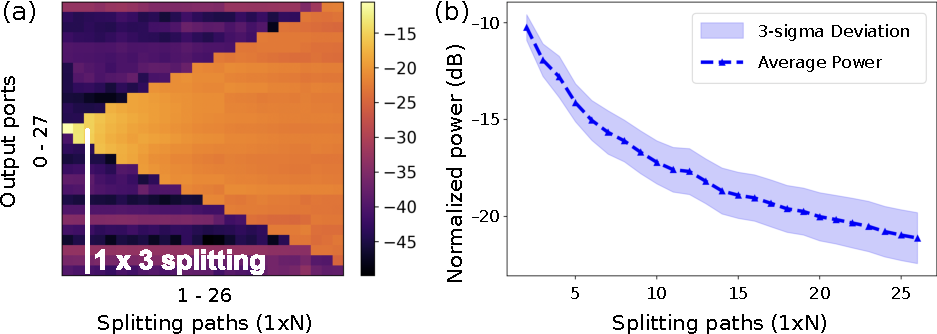
\includegraphics{figures/ch3-splitters_power_meter.pdf}
	\end{center}
	\caption{Optical beamsplitter demonstration: (a) Output power colormap as a function of
		the number of splitting paths starting from 2 (second leftmost column) and 26 (rightmost column).
		The white lines point to the measured output powers for the configuration in Fig.~\ref{fig:ch3-splitter}.
		We observe how the input laser power is evenly distributed across the output ports.
		In (b) we observe the average output power and its deviation with respect to the number of splitting paths.
	}\label{fig:ch3-splitters_power_meter}
\end{figure}

% section Beam splitters (end)

\section{Switches}\label{sec:switches} % (fold)

\begin{figure}
	\begin{center}
		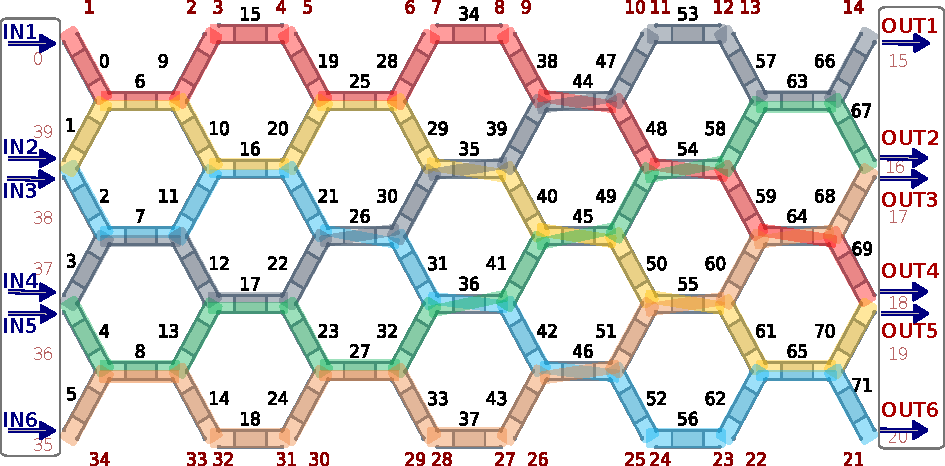
\includegraphics{figures/ch3-ocs.pdf}
	\end{center}
	\caption{Optical circuit switching experiment.
		Programmable processor 6x6 circuit switch configuration.
		Input ports 0, 39, 38, 37, 36, 35 and output ports 15, 16, 17, 18, 19, 20 are numbered from 1 to 6 each in blue color and red color respectively.
	}\label{fig:ch3-ocs}
\end{figure}

Optical circuit switching is a technology that allows to configure the physical layer of an optical network through software instructions.
It holds the potential to improve the cost, latency and power consumption used by ML/AI workloads within data centers \cite{khani_sip-ml_2021,liu_lightwave_2023,sato_prospects_2022}.
When the traffic circulating in a network is deterministic the physical layer can be used to route the data directly and the need for an Electronic Packet Switch (EPS) can be avoided.
In this section, we present the implementation of an on-chip software-defined switch that enables the dynamic control of optical waveguide paths for multiple input and output channels.
Such a system has been synthesized on the hexagonal core introduced previously and has been designed to cross-connect 6 pairs of inputs-outputs.
To enable the automatic configurability of the full 6-by-6 switch matrix we have adapted three algorithms and implemented them in our software stack.
The algorithms explored in this work are sequential routing \cite{lopez_auto-routing_2020}, graph-based with edge weight penalty \cite{kerchove_automated_2023}, and analytical decomposition \cite{jia_six-port_2018}.
The first two are more general as they make use of iterative algorithms to find the non-conflicting routes between the set of port pairs.
The first is the most time-consuming of the three as it relies on testing all possible I/O port routes until it finds a non-conflicting solution.
The edge penalty approach is an iterative algorithm that makes use of dynamic weight updates in the graph to penalize conflicting path sections.
Once the weight is updated the routine will attempt to find a new route in the next iteration.
The \lstinline|max_iter| parameter (see Listing~\ref{lst:ch3-ocs}) regulates the maximum number of iterations for path re-routing in instances of edge conflicts, when no routing solution exists for certain input/output port combinations.
The third approach is fully analytical and relies on the mathematical decomposition of the switch matrix to a Spanke-Bennes network synthesized on the hexagonal mesh.
The solution in this case is immediate due to the analytical nature of the problem, however, the set of hexagonal core ports that can be used are restricted by the feed-forward network architecture.
The latter statement means that only the ports on the west and east side of the mesh can be used by this method, whereas the north and south ports can only be included for the iterative ones.
Regarding switching speed, the device's reconfiguration time is primarily determined by the thermo-optic actuator, which operates on the scale of microseconds, compared to hundreds of milliseconds in the case of MEMs-based approaches \cite{poutievski_jupiter_2022,urata_mission_2022}.

\begin{lstlisting}[caption={Implementation of iterative and analytical switch networks using the first-generation Smartlight API}, label=lst:ch3-ocs]
# Iterative method
input_ports = [0, 1, 2, 3, 4, 5]
output_ports = [5, 1, 2, 3, 4, 0]
pucs_configuration = smart.auto_switch(
    input_ports, output_ports, max_iter=50 
)
# Analytical method
switch_config = {0: 5, 1: 1, 2: 2, 3: 3, 4: 4, 5: 0}
feedforward = smart.feedforward_operator(dim=6, puc_0=0)
feedforward.load_switch_config(switch_config)
smart.load_feedforward_config(feedforward)
\end{lstlisting}

The first and third approaches are straightforward to implement and have been previously documented \cite{lopez_auto-routing_2020,jia_six-port_2018}.
The second approach was developed by iPronics and is detailed in depth in \cite{xie_software-defined_2024}.
The edge penalty algorithm has the advantage of being more efficient than the brute force algorithm (first approach) and more flexible than the third as it is not constrained to the ports of a Spanke-Bennes network.
Refer to Listing~\ref{lst:ch3-ocs} for the implementation of a 6-by-6 switching network using the iterative and analytical approaches, respectively.
The iterative one implements the weight-penalty/re-routing algorithms while the analytical method relies on the Clements decomposition of unitary switch matrix operators which will be covered in detail in Chapter~\ref{chap:universal_unitary_operators}.
% In lines 1 and 2, the best paths for each I/O port pair are identified.
% The next step is to check whether these paths contain conflict edges (line 4), as conflicting edges within the identified paths will be penalized with a higher weight (line 6).
The iterative method relies on identifying conflicting edges within a switch network and finding alternative paths to circumvent the conflicting zones.
What we define as a conflicting edge is a PUC that belongs to two or more paths and has a different state (cross/bar) in at least two of these paths.
A switching network needs to have zero conflicting edges to work.
% Once the problematic edges have been penalized, we recompute new optimal paths for the I/O ports pairs considering the new edge weights and updating the preprocessing paths configuration list (line 7, 8).
The algorithms iterate until the conflicts across the network have been solved.
If no conflicts are detected, the configuration of optimal paths will be saved and the loop will be stopped, otherwise the iterative process of weight update will continue until a zero-conflict configuration is found or the max number of iterations is reached.
If the number of iterations goes beyond the \lstinline|max_iter| value, the problem will be considered unsolved.
Hence, this variable represents the trade-off between the probability of finding a solution and the time spent searching for a zero-conflict configuration.
As mentioned before, the analytical method ensures the existence of a solution under the condition that only the input/output ports of a feedforward operator (e.g., the ones in blue/red in Fig.~\ref{fig:ch3-ocs} for an operator of size $N=6$) are used.
The rest of the hexagonal mesh ports would remain idle.
As stated previously, if there's a need to use other hexagonal mesh ports then the iterative algorithms are the ones to go with.
This particular case might be useful for some testing/prototyping applications that require additional flexibility.

In Figure~\ref{fig:ch3-ocs} we present the implementation of a 6x6 optical circuit switch with the different paths painted in different colors and all PUCs activated.
Notice that we have selected six ports from the left side of the hexagonal mesh [0, 27, 26, 25, 24, 23] as inputs and other six ports from the right side [15, 16, 17, 18, 19, 20] as outputs, the selected ports from both sides are named from 1 to 6 in blue color and red color, respectively.
To measure the performance of the network, six distinct switch configurations have been implemented using a laser source with 5 dBm input power connected to port 1.
The switch was then programmed to synthesize 6 different configurations between this input and all the possible outputs.
With the network defined, the power of each output port was measured and normalized with the input source, resulting in the characterization of 6 switch matrices.
The process was repeated for the other 5 inputs leading to the characterization of 36 switch matrices in total.
We denote that due to limited lab equipment at the time we characterized the switch by looking one input port at a time.
This means that, when all input ports are populated the total optical crosstalk will be slightly higher than the reported value (\(\approx [22,25]\) dB).
Nevertheless, later trials with six laser signals confirm that the 6-to-6 switch correct functioning holds \cite{sanchez-jacome_parametric_2024}.

In Figure~\ref{fig:ch3-ocs_power_meter} we present the measured results.
Here, each column in the subfigure represents the optical power monitored in a specific output port, and the different marker shapes correspond to the 6 different input ports.
Our results demonstrate the optical circuit switch’s performance showcasing accurate switching of multiple inputs to their respective target outputs.
Notably, the distances of all switch circuit paths are consistent, passing through 15 PUCs.
As a result, we observed -10 dB (± 0.5) insertion losses in all 6 output ports for each configuration.
The Attenuation-to-crosstalk ratio (ACR) is determined by checking the difference between the optical power from the specified input output pair and the highest leakage power from other input ports to the same output port.
This distinction is visually represented by the distance between two blue lines in Fig.~\ref{fig:ch3-ocs_power_meter}, with a typical value of 25 dB.
This metric varies based on the switch configuration, the best scenario of crosstalk observed in our experiments is 26 dB for the switch configuration: [1:4, 2:5, 3:6, 4:1, 5:2, 6:3].
The source of crosstalk is mainly from PUC performance, as well as small drifts due to auto-calibration and auto-characterization.
% ===Leaving reconf time out to avoid having conflicts of interest with iPronics ===
% The reconfiguration speed can be broken down in physical layer reconfiguration, control plane latency and algorithm computation time as shown in Table 2.
% Physical layer latency independent of number of elements to be tuned but control plane scaling linearly with number of PUCs.
% Software plane time ranges from milliseconds to seconds based on algorithm choice, in which edge penalty and sequential routing approaches take more time as they require a conflict-edge resolution step.

% Table 2.
% Configuration speed of optical switch circuit
%
% Latency (ms) Physical layer 0.18 Control plane 48 Algorithm Computation 38 (1) 2700 (2) 5800 (3) Total 86.18 (1) 2748.18 (2) 5848.18 (3)
%
% (1) Analytical decomposition.
% (2) Edge penalty algorithm. (3) Sequential routing
% ===Leaving reconf time out to avoid having conflicts of interest with iPronics ===

Using the same set of selected I/O ports, we evaluate the feasibility of the algorithm.
For the 6x6 circuit switch, there are a total of \(6!
=720\) possible combinations, representing distinct switch circuits for both, iterative and analytical algorithms.
The switching architecture can be classified as rearrangeable non-blocking as it needs to reconfigure already established connections to allocate new ones.
The algorithm demonstrated its reliability by generating feasible solutions for all 720 cases without any observed instances of failure.
This fact makes the software layer developed for this work a key differentiator with respect to previous manually implemented solutions.

\begin{figure}
	\begin{center}
		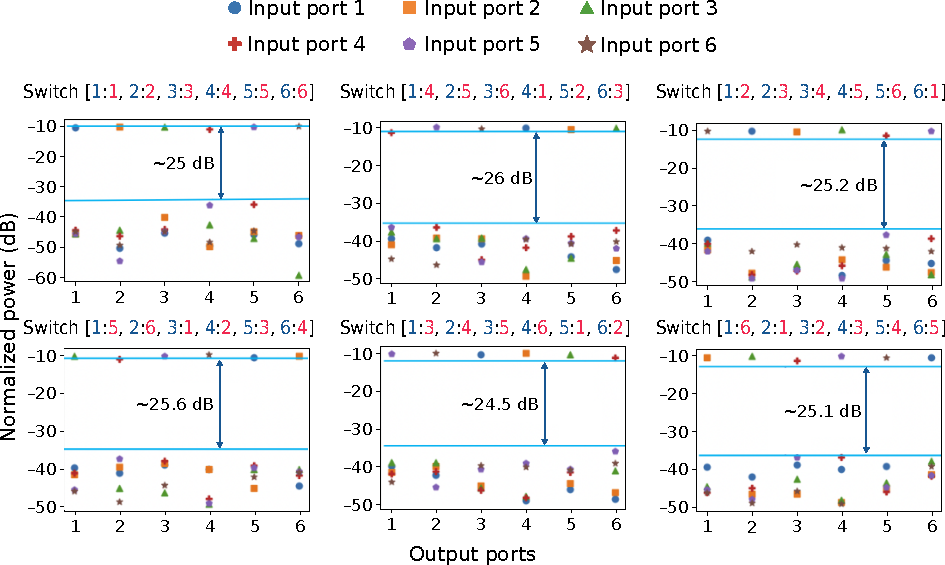
\includegraphics{figures/ch3-ocs_power_meter.pdf}
	\end{center}
	\caption{Optical circuit switching demonstration:
		6-by-6 switch matrix for 6 different configurations.
		Each subplot demonstrates the output of a specific switch configuration, with the X-axis depicting the output ports in the mesh and the Y-axis representing the measured optical power levels at the output ports.
		The six input ports are visually represented by six distinct markers in the figure.
	}\label{fig:ch3-ocs_power_meter}
\end{figure}

% section Switches (end)

\section{Filters}\label{sec:filters} % (fold)

% Tunable and reconfigurable photonic filters
The first-generation Smartlight photonic processor has the ability to implement various types of tunable and reconfigurable photonic filters.
These filters are crucial for microwave photonics (MWP) applications, as they allow precise signal shaping, noise reduction, and channel selection in the radiofrequency (RF) domain \cite{marpaung_si3n4_2013,liu_integrated_2020,daulay_tutorial_2021}.
In traditional systems, photonic filters are fixed-function devices or require bulky, discrete optical components.
The programmable photonic processor overcomes these limitations by offering on-chip tunable filters, implemented through software-controlled photonic circuits.
This platform can implement multiple types of tunable filters, including finite impulse response (FIR) filters such as unbalanced Mach-Zehnder interferometers (UMZIs) and lattice filters.
The same applies to infinite impulse response (IIR) such as optical ring resonators (ORRs), ring-assisted Mach-Zehnder Interferometer (RAMZI) filters, coupled resonant waveguide (CROW) filters, side-coupled integrated spaced sequence of optical resonators (SCISSORS) of multiple orders.
These filters are realized through the hexagonal waveguide mesh with 72 PUCs and the filter's order is limited by this core size.

\begin{lstlisting}[caption={Implementation of IIR and FIR optical filters using the first-generation Smartlight API}, label=lst:ch3-filters]
# IIR Filter 
smart.reset_mesh()
# 3rd order CROW
crow = [
    (1, "="), (2, k1), (6, "="), (7, "="), (9, "="), (10, k2),
    (11, "="), (15, "="), (16, "="), (19, "="), (20, k3),
    (21, "="), (25, "="), (26, "="), (28, "x"), (29, k4),
    (30, "="),
]
# 2nd order:
# [(28, "x")], 25 -> inactive
# FIR Filter 
smart.reset_mesh()
lattice = [
    (1, "="), (2, "x"), (3, k5), (6, "="), (7, "x"), (10, "x"),
    (11, "x"), (16, k6), (20, "x"), (21, "x"), (25, "="),
    (26, "x"), (29, "="), (30, "x"), (31, k7), (32, "x"),
    (33, "="), (36, "x"), (37, "="), (42, "x"), (43, "x"),
    (46, k8), (47, "x"), (48, "x"), (49, "x"), (50, "x"),
    (51, "="),
]
puc_info = crow # lattice 
smart.filter(puc_info)
\end{lstlisting}

\begin{figure}[t!]
	\begin{center}
		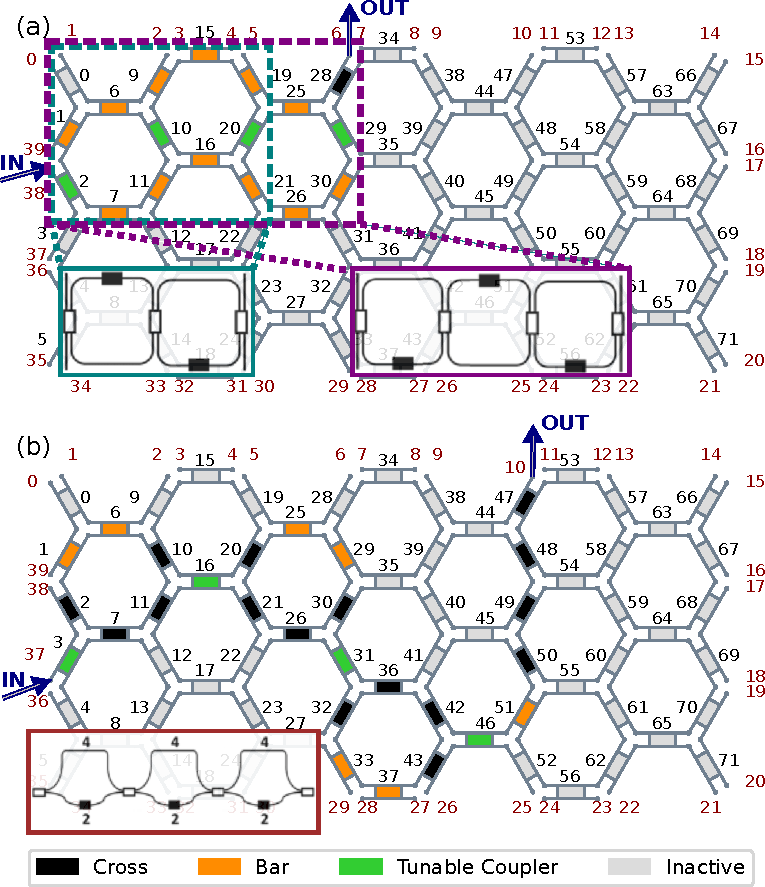
\includegraphics{figures/ch3-filters.pdf}
	\end{center}
	\caption{Optical filtering experiment.
		(a) Circuit schematic and waveguide mesh implementation of resonant (IIR) second (turquoise) and third-order (purple) CROW filters featuring coupled-ring cavities of length 6~BUL.
		(b) Circuit schematic (red box) and waveguide mesh implementation of a third-order UMZI photonic lattice filter.
	}\label{fig:ch3-filters}
\end{figure}

To demonstrate the capabilities of the programmable photonic processor, we configured the photonic waveguide mesh to implement various filter architectures and tested their performance.
The experiments demonstrated the implementation of multiple tunable filters.
The implementation of one IIR and one FIR filter is presented in Listing~\ref{lst:ch3-filters} using the developed Python API.
For the IIR case we synthesized a second (turquoise) and third-order (purple) resonant Coupled Resonant Optical Waveguide (CROW) filters, which consisted of two and three coupled-ring cavities, respectively, (see Figure~\ref{fig:ch3-filters}(a)).
These filters have two complementary outputs representing the through and drop responses of a resonant filter (refer to Section~\ref{sub:integrated_photonic_resonant_devices}).
The through response of the second-order CROW, in Fig.~\ref{fig:ch3-filters_osa}(a), exhibits a notch response with a suppression of 26 dB and a free spectral range (FSR) of 14.98 GHz.
The drop spectrum of the third-order CROW is shown in Fig.~\ref{fig:ch3-filters_osa}(b).
As expected, we observe a band-pass characteristic with an extinction ratio of 23 dB.
We notice that in this case the inclusion of another ring has increased the insertion losses of the circuit in around 10 dB.
These losses can be reduced by improving the tuning and resolution of coupling between the rings, so signal leakage can be minimized.
The right part of Figure~\ref{fig:ch3-filters_osa}(b) shows the band-pass tuning along a complete FSR where the resonance frequency could be tuned by modifying cross-phase shifters in the intracavity PUCs.
For the FIR case we implemented a third-order UMZI lattice filter (see Figure~\ref{fig:ch3-filters}(b)).
The latter exhibits a band-pass response with an extinction ratio of 21 dB and FSR of 44.95 GHz as shown in Figure~\ref{fig:ch3-filters_osa}(c) left.
This filter was fully tunable over an entire FSR interval by reconfiguring cross-phase shifters (see Fig.~\ref{fig:ch3-filters_osa}(c) right).
Both filters can be optimized by tuning the internal PUC responses and changing the zero and pole positions \cite{madsen_digital_1999}.
In \cite{perez-lopez_supplementary_2024} we provide a detailed description of the implementation and measurements of 17 additional types of filter architectures.

\begin{figure}[t!]
	\begin{center}
		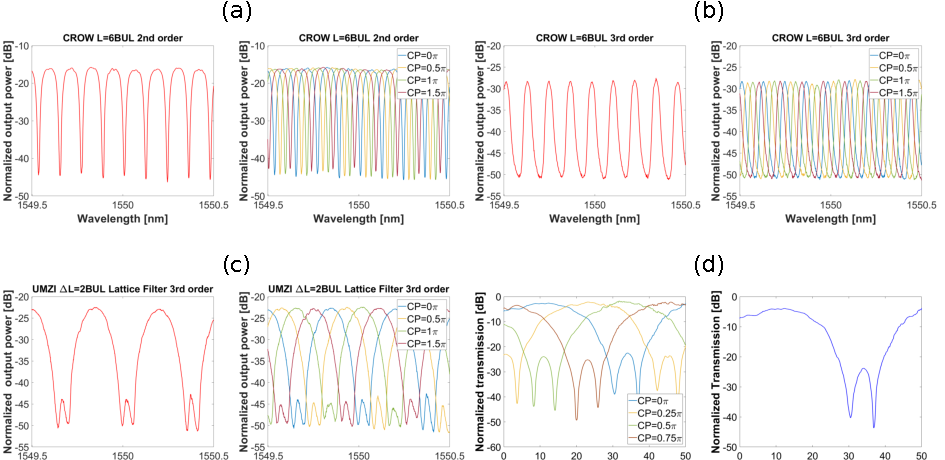
\includegraphics{figures/ch3-filters_osa.pdf}
	\end{center}
	\caption{Optical filtering demonstration.
		Third-order CROW filter featuring three coupled-ring cavities of length 6BUL: (a) Left: Spectral response for the reflection spectrum.
		Right: frequency notch tuning along a complete FSR (using an intracavity PUC as a cross-phase shifter CP).
		(b) Left: Transmission spectrum,  Right: band-pass tuning along a complete FSR (using an intracavity PUC as a cross-phase shifter CP).
		(c) Optical transfer function and the tuning of the UMZI lattice filter and (d) RF transfer function and the tuning of the MWP filter based on self-beating of the third-order UMZI photonic lattice filter. }\label{fig:ch3-filters_osa}
\end{figure}

\begin{figure}[htb]
	\begin{center}
		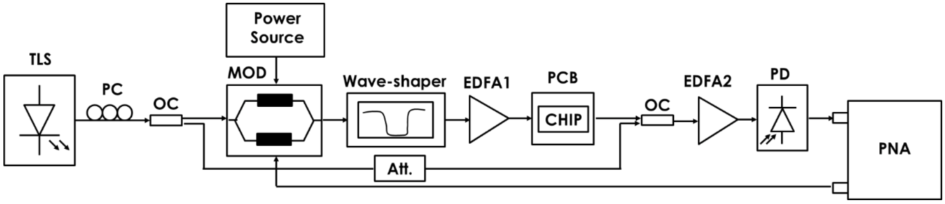
\includegraphics{figures/ch3-filters_rf_conversion.pdf}
	\end{center}
	\caption{Passive setup used to measure the radiofrequency response of the different optical filters.
	}\label{fig:ch3-filters_rf_conversion}
\end{figure}

% Tunable and reconfigurable radiofrequency filters and phase shifters
The radiofrequency response of these optical filters can be obtained from direct down-conversion of their spectrum.
For this, an input single-sideband RF signal must be employed, the optical carrier must be suppressed, re-injected and combined with the upconverted RF sideband after the latter is processed by the filter.
As depicted in Figure~\ref{fig:ch3-filters_rf_conversion}, first, an optical carrier emitted by a tunable laser source (TLS), and a vector network analyzer (PNA, Optical Network Analyzer) is used to modulate the electro-optic modulator biased at the quadrature bias point (QB).
A dual-drive modulator (MOD) was used as a modulator, in combination with a wave-shaper, implementing a stop-band filter to implement the carrier suppression and single- sideband modulation.
In addition, we used two optical couplers (OC) at the input (50/50) and output (50/50) to implement the self-beating technique.
The SSB modulated signal is amplified by an erbium-doped fiber amplifier (EDFA) from and introduced to the optical integrated filter synthesized in the photonic mesh.
Once the signal is outside the chip, it is amplified again with another EDFA for compensating the losses suffered in the integrated chip, and photo detected and sent to the microwave network analyzer (PNA) to measure the transmission response.

% We assembled a testing and measurement setup as described in Supplementary Note 5 to measure the implementation of MWP filters based on different photonic filters.
Figure~\ref{fig:ch3-filters_osa}(d) shows the transfer function and the tuning of an MWP filter based on the third-order UMZI photonic lattice filter described previously.
Note that the filter displays an RF power extinction ratio of 40 dB and features a radiofrequency FSR of 44 GHz (matching its photonic counterpart).
The interested reader is directed to Supplementary Note 5 of \cite{perez-lopez_supplementary_2024} for the implementation details of other microwave photonic filters.
It is important to highlight here that, when compared to application-specific photonic circuits, the programmable processor suffers from extra excess losses due to the waveguide lattice mesh, reducing the total RF gain of the filter.
To overcome this limitation, the integration of optical amplifiers in the system can be considered as discussed in Section~\ref{sub:amplification}.

% section Filters (end)

\section{Reconfigurable delay lines}\label{sec:reconfigurable_delay_lines} % (fold)

True time optical delay lines (TTODLs) are important because they enable precise, dynamically adjustable delays in photonic circuits, which are essential for advanced microwave photonics applications \cite{lenz_optical_2001,xiang_low-loss_2018,zhu_silicon_2020}.
By providing a means to finely control signal timing and phase, TTODLs are instrumental in beamforming networks where accurate synchronization of signals across an antenna array is vital for steering beams without distortion or squint.
% The latter capability is particularly important for wideband applications in next-generation wireless communications, radar, and optical filtering.
TTODLs solve the beam squint problem by providing frequency-independent phase shifting, which ensures that signals at different frequencies experience the same time delay.
In traditional phased array systems that use phase shifters, the delay introduced is proportional to the signal's wavelength.
This is solved by introducing actual path differences between the signals so that a constant time delay is introduced instead of a phase shift.
Moreover, integrating TTODLs into waveguide mesh architectures offers significant advantages over traditional static delay lines.
As proposed by \cite{perez-lopez_programmable_2018}, it allows for a compact, reconfigurable, and programmable platform that can adapt to varying system requirements in real time.

\begin{figure}[t!]
	\begin{center}
		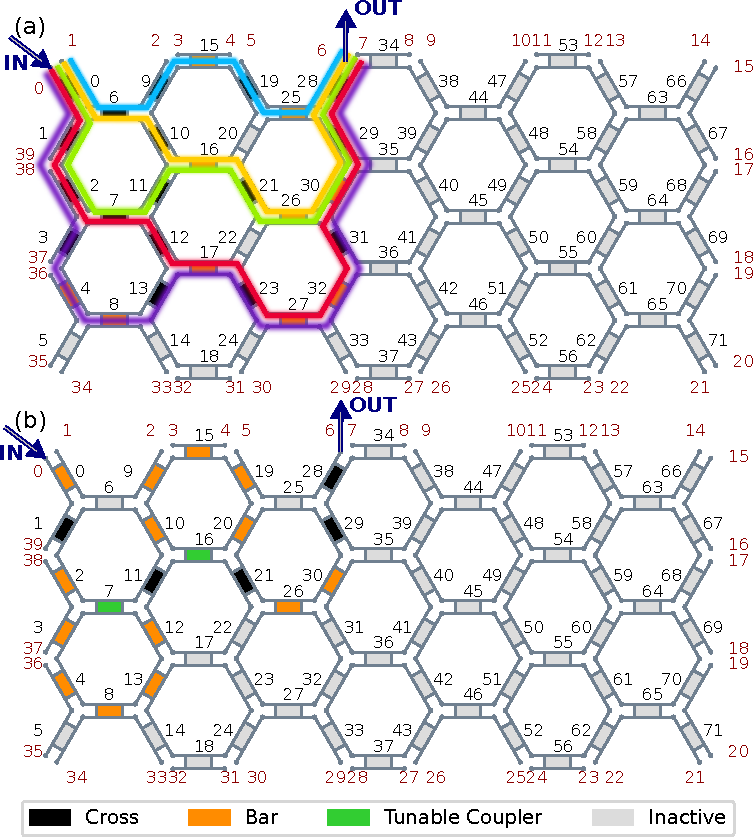
\includegraphics{figures/ch3-delay_circuits.pdf}
	\end{center}
	\caption{Optical delay lines experiment.
		(a) Schematic of discrete delay lines on the hexagonal mesh using port 0 and 6 as input and output, respectively.
		Longer paths are used to introduced higher delays.
		(b) Schematic of a SCISSOR filter used to generate a continuous delay response between discrete steps.
	}\label{fig:ch3-delay_circuits}
\end{figure}

In this work we present the implementation of discrete and continuous delay lines on the iPronics first-generation Smartlight platform.
The code implementation of both can be found in Listing~\ref{lst:ch3-delay_circuits} where both discrete and continuous circuits are detailed.
The first are represented by the overlap of interconnect paths of different lengths with a minimum \(\Delta L = 2\cdot BUL\) (or \(\Delta \tau = 2\cdot \tau_{BUL}\)) where \(BUL = 811.41 \mu m\) (or \(\tau_{BUL} = 11.25 ps\)).
The \(2\cdot \) constrain emerges from the hexagonal architecture.
The time delay performance of each path was measured with the processor fed with an input pulsed signal from a LUNA optical vector analyzer (OVA).
The different paths configurations were programmed on the processor and their time responses measured with the OVA which provided the amplitude and delay characteristics of each input/output port pair.
As observed in Figure~\ref{fig:ch3-delay_luna}(a), the peak response of the different paths are consistently spaced by \(22.5\,ps\) as expected, with their responses only being different by a decreasing peak amplitude.
The latter occurs due to the increasing insertion losses of adding 2 more PUCs to each longer path.
Recall that the reported losses of this platform are \(IL_{PUC} \approx 0.46\) dB.
\\ % New linte to avoid splitting listing

\begin{lstlisting}[caption={Configuration of discrete and continuous delay lines using the first-generation Smartlight API}, label=lst:ch3-delay_circuits]
	# Discrete delays
	delay_1 = [
		(0, "x"), (6, "="), (9, "x"), (15, "="), (19, "x"), (25, "="),
		(28, "="),
	]
	delay_2 = [
		(0, "x"), (6, "x"), (10, "x"), (16, "x"), (21, "x"), (26, "="),
		(30, "="), (29, "x"), (28, "x"),
	]
	# Continuous delay
	scissor = [
		(0, "="), (1, "x"), (2, "="), (7, k1), (12, "="), (13, "="),
		(8, "="), (4, "="), (3, "="), (11, "x"), (16, k2), (10, "="),
		(9, "="), (15, "="), (19, "="), (20, "="), (21, "x"), (26, "="),
		(30, "="), (29, "x"), (28, "x"),
	] % k1=k2=0.05
	puc_info = scissor # delay_1+delay_2
	smart.manual_circuit_configuration(puc_info)
	set_coupling_factor_phase([(8, ["=", cp]), (15, ["=", -1*cp])])
\end{lstlisting}

\begin{figure}[h]
	\begin{center}
		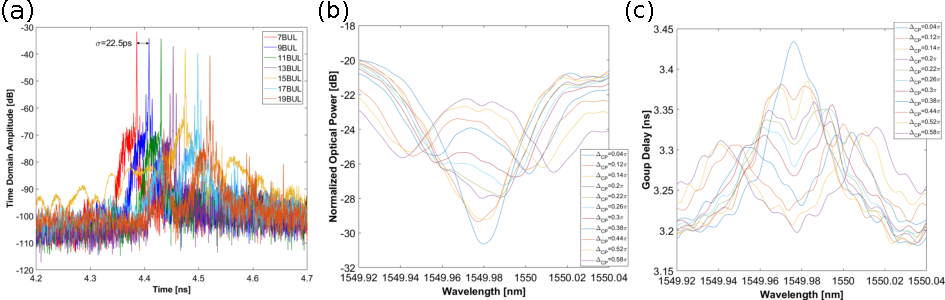
\includegraphics{figures/ch3-delay_luna.pdf}
	\end{center}
	\caption{Reconfigurable delay line demonstration.
		(a) Discrete time delay steps observed through an optical vector analyzer (OVA) with steps of 22.5~ps observed.
		(b) Transmission response of the SCISSOR circuit when applying different cross-phases to detune the resonance wavelengths of its inner rings in order to achieve different group delay responses.
		(c) Continuous time delay yielded by detuning the rings of a SCISSOR circuit through different cross-phases.
		Different values of cross-phases lead to different values of group delay at the transmission port.
		The continuous delay is observed to cover a span of 0.24~ns.
	}\label{fig:ch3-delay_luna}
\end{figure}

The continuous delay demonstration is performed by synthesizing the SCISSOR circuit in Listing~\ref{lst:ch3-delay_circuits}.
To measure the time response we employed the OVA connected to both the input and output of the SCISSOR structure.
The first step was to tune both rings so that their resonances match.
To achieve this, we use the \lstinline|set_coupling_factor_phase()| instruction on PUCs 8 and 15 to perform the fine-tuning until reaching the resonant point (See Fig.~\ref{fig:ch3-delay_luna}(b) for \(\Delta_{CP}=0.04 \pi \)).
From here we performed a detuning of the rings by adding an asymmetric offset to the cross-phases of PUCs 8 and 15.
When this detuning happens the amplitude response of the filter changes and, due to the dispersive nature of this structure, its group delay also changes.
This effectively introduces a continuous delay line which can be controlled by the cross-phase tuning.
In Figure~\ref{fig:ch3-delay_luna}(c), we observe that the maximum continuous delay span that can be obtained with this method is of 0.24~ns, which is more than enough to fill the discrete steps presented in the discrete example.
A combination of both discrete and continuous delay lines could be implemented on a larger mesh with more recirculating cells where each arm can be loaded by a SCISSOR structure.
This would enable smooth beam steering applications where the coarse delay is added with interconnect paths and the fine delay is inserted by the ring detuning.
Certainly, such a large scale solution will require that PUCs are small so that insertion losses, time step \(\Delta_{BUL}\) and area can be minimized \cite{perez-lopez_integrated_2019}.
We also denote that the loss penalty for introducing the continuous delay can reach \(\approx 9\) dB for the entire 0.24~ns span.
However, it's important to consider that in order to cover the full range between two discrete delay steps (22.5~ps), the expected loss is \(\approx 1\) dB, which is comparable to the discrete step penalty.

% section Continuous delay lines (end)

\section{Topological photonic arrays}\label{sec:topological_photonic_arrays} % (fold)

\begin{figure}[b!]
	\begin{center}
		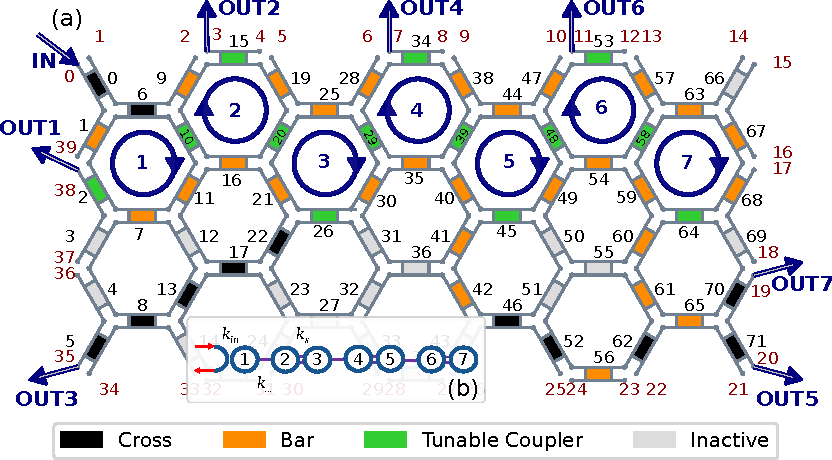
\includegraphics{figures/ch3-topological-ssh.pdf}
	\end{center}
	\caption{(a) Implementation of the Su-Schrieffer-Heeger (SSH) model circuit using seven ring resonators and optical paths to tap out signal power. (b) Schematic of the implemented 1D SSH model.}\label{fig:ch3-topological_ssh}
\end{figure}

% In this section we explore the use of programmable photonic circuits to implement topological Hamiltonians within a single reconfigurable platform \cite{on_programmable_2024}.
Topological photonics can trace its roots to the discovery of topological insulators in condensed matter physics \cite{klitzing_new_1980,thouless_quantized_1982}, where bulk materials that are naturally insulating can conduct electricity under certain conditions.
These concepts have been replicated in the photonics world \cite{ozawa_topological_2019,price_roadmap_2022}, where topology refers to a quantized property that describes the global behavior of the wavefunctions in a dispersion band.
A key feature of topological photonics is the existence of modes that live on the edge of photonic materials with non-trivial topologies and that show resilience to certain types of disorder.
While topological photonics has led to significant advancements in areas such as lasing, sensing, and quantum technologies \cite{shalaev_robust_2019,bahari_nonreciprocal_2017,ezawa_higher-order_2018,blanco-redondo_topological_2018}, existing experimental implementations typically support only fixed topological models with limited or no reconfigurability.
Here, we document how this limitation can be overcome by using the first-generation Smartlight programmable silicon photonic mesh to allow real-time control of key parameters such as hopping strengths, phase shifts, and on-site potentials.
This reconfigurable approach positions programmable photonics as a universal testbed for exploring topological physics and novel photonic devices, accelerating research in non-Hermitian photonics, quantum optics, and programmable photonic computing.
In \cite{on_programmable_2024}, we demonstrate the versatility of this approach by experimentally implementing the 1D Su-Schrieffer-Heeger (SSH) model, which supports robust edge states, and simulating the 2D breathing Kagome lattice, which hosts higher-order topological corner states.
In this section we present the circuit and the experimental results obtained from the former model.

The Su-Schrieffer-Heeger is the simplest topological model \cite{su_solitons_1979}.
It's a dimmer chain which is composed by an alternate pattern of weak and strong coupling between sites.
Here, we implement the SSH model in the hexagonal mesh by configuring it as a bipartite lattice of seven ring resonators connected with one another as shown in Fig.~\ref{fig:ch3-topological_ssh}(b).
The equivalent synthesized circuit on the programmable mesh is marked by blue circumferences in Fig.~\ref{fig:ch3-topological_ssh}(a).
The Python code needed to implement this circuit on the programmable core is presented in Listing~\ref{lst:ch3-topological_ssh}.

The Hamiltonian describing this system of rings is given by

\begin{equation}
	H = \left[ k_w \sum_{n \in \{1,3,5\}} a_n^\dagger a_{n+1} + k_s \sum_{n \in \{2,4,6\}} a_n^\dagger a_{n+1} \right] + H.c.
	\label{eq:ch3-topological_ssh}
\end{equation}

where $k_w$ and $k_s$ are the strong and weak coupling strengths between sites, and $a_n^\dagger$ and $a_n$ are the creation and annihilation operators on site $n$.
Note that these variables are directly translated to the coupling factor settings in Listing~\ref{lst:ch3-topological_ssh}.
Also notice that optical paths have been configured on the mesh to tap some power from the rings using the on-chip photodetectors.
Specifically, 1\% of the power is coupled out using PUCs as couplers.

\begin{lstlisting}[caption={Implementation of the Su-Schrieffer-Heeger (SSH) model using the first-generation Smartlight API}, label=lst:ch3-topological_ssh]
rings = [ 
    (0, "x"), (1, "="), (2, 0.01), (6, "x"), (7, "="), (9, "="),
    (10, k_w), (11, "="), (15, 0.01), (16, "="), (19, "="),
    (20, k_s), (21, "="), (25, "="), (26, 0.01), (28, "="),
    (29, k_w), (30, "="), (34, 0.01), (35, "="), (38, "="),
    (39, k_s), (40, "="), (44, "="), (45, 0.01), (47, "="),
    (48, k_w), (49, "="), (53, 0.5), (54, "="), (57, "="),
    (58, k_s), (59, "="), (63, "="), (64, 0.01), (67, "="),
    (68, "="),
]
pd_paths = [
    (5, "x"), (8, "x"), (13, "x"), (17, "x"), (22, "x"), (41, "="),
    (42, "="), (46, "x"), (52, "x"), (56, "="), (62, "x"),
    (60, "="), (61, "="), (65, "="), (70, "x"), (71, "x"),
]
su_schrieffer_heeger = rings + pd_paths
smart.manual_circuit_configuration(su_schrieffer_heeger)
\end{lstlisting}

Figure~\ref{fig:ch3-topological-power_meter} shows that by configuring the mesh into a dimerized lattice and alternating the coupling strengths between sites (using the coupler PUCs to set $k_w$ and $k_s$), we enable the formation of topologically protected edge states.
The calculated eigenvalues of this lattice, represented here by the resonant frequencies of the supermodes, are shown in Figure~\ref{fig:ch3-topological-power_meter}(a) for four different combinations of $k_w$ and $k_s$, which is referred as the dimerization pattern from now on.
The experimental measurements in Figure~\ref{fig:ch3-topological-power_meter}(b) confirms that in the topological phase, light remains strongly localized at the system’s boundary, while virtually zero power is measured in the even rings.
The robustness of the edge state is further tested by introducing disorder in the coupling strengths, showing that the topological mode persists even under perturbations.
Figure~\ref{fig:ch3-topological-power_meter}(c-d) shows the power sum in all the even and odd rings when the input laser is swept $\pm$ 6 GHz from its central frequency $f_0=193 THz$.
Here, we observe that stronger dimerization patterns lead to larger band gaps and more pronounced edge localization.
This is because the only supermode supported around $f_0$ is the topological edge mode, which is fully localized in the odd rings.
The residual amount of power observed in the even rings at f0 is due to the non-perfect overlap of the input light with the modal profile of the edge mode.
These results highlight the ability of the programmable platform to precisely tune topological properties.

\begin{figure}
	\begin{center}
		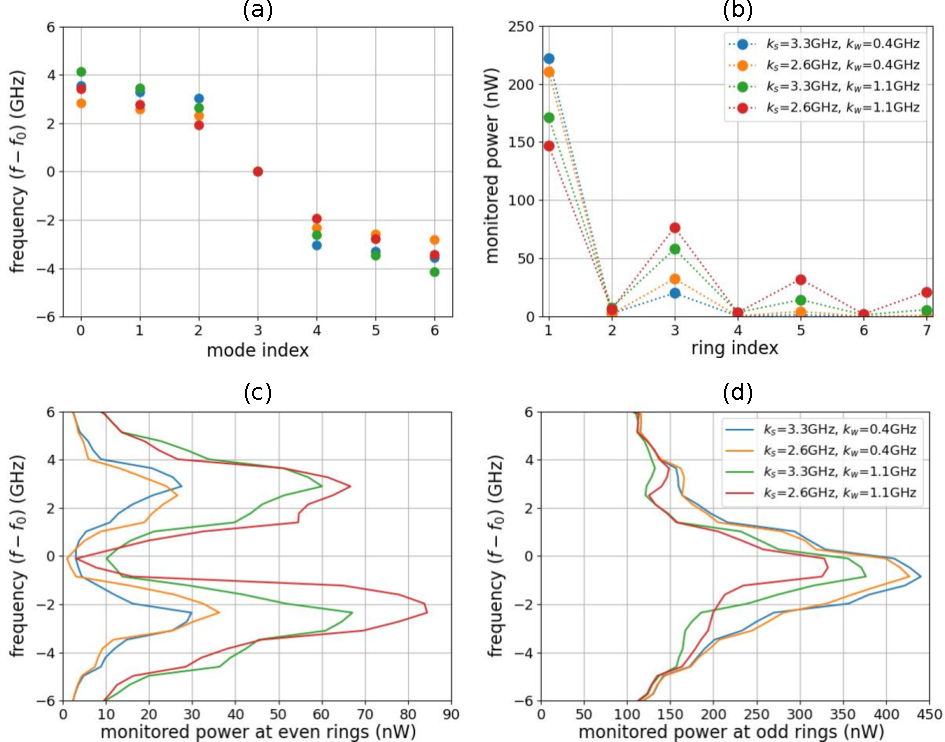
\includegraphics{figures/ch3-topological-power_meter.pdf}
	\end{center}
	\caption{Characterization of the eigenvalues and the topological edge mode in the SSH model. (a) Calculated eigenvalues of the Hamiltonian matrices. (b) Monitored powers (tapped ≈ 1\% of the power in
		each ring) at the coupled ring resonators from the programmable mesh hardware. (c) Total monitored power (tapped ≈ 1\%) spectrum of the even rings of 1D SSH model. (d) Total monitored power spectrum
		of the odd rings of 1D SSH model.}\label{fig:ch3-topological-power_meter}
\end{figure}

% section Topological photonic arrays (end)

\section{Optical Max Pooling}\label{sec:optical_max_pooling} % (fold)

\begin{figure}[b!]
	\begin{center}
		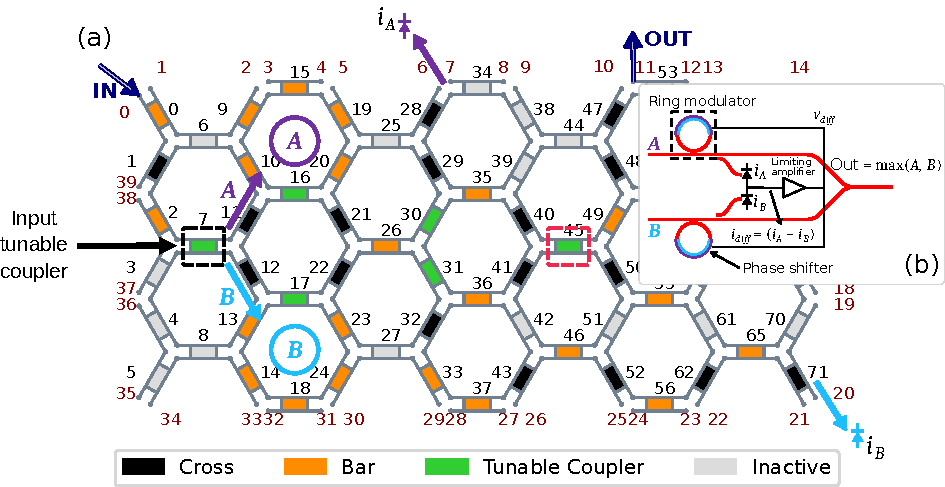
\includegraphics{figures/ch3-maxpool-circuit.pdf}
	\end{center}
	\caption{(a) Implementation of the proposed max pooling circuit on a programmable photonic platform.  (b) Proposed max pooling architecture using integrated ring modulators}\label{fig:ch3-maxpool-circuit}
\end{figure}

PICs have attracted attention as a solution to address the growing computational demands of deep neural networks (DNNs) and the limitations of traditional digital hardware, such as GPUs, as a platform to reduce power consumption and improve computational speed.
Experimental demonstrations of the building blocks of neural networks such as multiply and accumulate (MAC) \cite{feldmann_parallel_2021,tait_neuromorphic_2017,ashtiani_-chip_2022} and all-optical/optoelectronic activation functions \cite{jha_reconfigurable_2020} have been published as standalone and system solutions.
The former MAC case and its implementations in a programmable photonic platform will be discussed in detail in Chapter~\ref{chap:universal_unitary_operators}.
Here we cover the optoelectronic implementation of a popular activation function: Pooling.
Pooling layers are used to downsample an input tensor by calculating the average (average-pooling) or maximum (max pooling) of its components.
Max pooling is commonly used to reduce computation load, improve feature extraction, and enhance invariance to input transformations \cite{murray_generalized_2014,zhang_winner-take-all_2020}.
While average pooling can be easily implemented using linear optical components, max pooling requires nonlinear processing making it difficult to implement directly using passive integrated components.
In this section we address this challenge by using optical ring modulators whose resonance conditions dynamically shift based on input power differences, effectively allowing the system to select the maximum input value \cite{ashtiani_photonic_2023}.

Figure~\ref{fig:ch3-maxpool-circuit} shows the proposed circuit synthesized on the programmable core alongside its target schematic.
Note that the circuit relies on an optoelectronic feedback loop to drive the ring modulators so that their notch responses are used to either suppress (discard) or pass (pool) one of the two input signals $(A,B)$.
Initially the rings' resonances are tuned and positioned symmetrically around \(\lambda_0\) so that the two signals go through.
A small fraction of the optical power from each ring is tapped using tunable couplers and sent to the on-chip photodetectors (PDs).
The PDs measure the power of each signal and are arranged to yield the proportional electrical current difference \(i_{diff} = i_A - i_B\).
This difference current is then amplified using a limiting amplifier, which ensures that the output voltage is constrained to two discrete levels, \(V_A\) and \(V_B\) which bring each ring resonance to \(\lambda_0\) and induce strong attenuation.
If \(A>B\) (\(B>A\)), the system shifts the resonance of ring \(B\)($A$) to align with \(λ_0\), heavily attenuating \(B\)($A$) while allowing \(A\)($B$) to pass.

\begin{equation}
	\text{Output} = \max(A, B)
	\label{eq:ch3-maxpool}
\end{equation}

The closed-loop feedback system ensures that even small differences between \(A\) and \(B\) are detected, making the system highly sensitive.
Since one ring is always locked to the operation wavelength \(λ_0\), the architecture remains stable and resistant to external perturbations or drift.

\begin{lstlisting}[caption={Impementation of an optical max pooling architecture using the first-generation Smartlight API.}, label=lst:ch3-maxpool-circuit]
maxpool_rings = [
    (0, "="), (1, "x"), (2, "="), (7, k_in), (9, "="), (10, "="),
    (11, "x"), (12, "x"), (13, "="), (14, "="), (15, "="),
    (16, 0.5), (17, 0.5), (18, "="), (19, "="), (20, "="),
    (21, "x"), (22, "x"), (23, "="), (24, "="), (26, "="),
]
maxpool_pds = [
    (28, "x"), (29, "x"), (30, 0.01), (31, 0.01), (32, "x"), (33, "="),
    (35, "="), (36, "="), (37, "="), (40, "x"), (41, "x"), (43, "x"),
    (45, 0.5), (46, "="), (47, "x"), (48, "x"), (49, "="), (50, "x"),
    (52, "x"), (55, "="), (56, "="), (60, "x"), (62, "x"), (64, "x"),
    (65, "="), (68, "x"), (71, "x"),
]
maxpool = maxpool_rings + maxpool_pds
smart.manual_circuit_configuration(maxpool)
\end{lstlisting}

\begin{figure}[b!]
	\begin{center}
		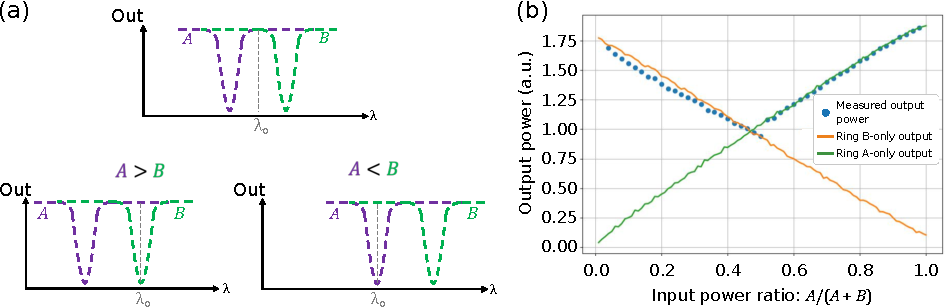
\includegraphics{figures/ch3-maxpool-power_meter.pdf}
	\end{center}
	\caption{
		(a) Expected the transfer characteristics of the proposed max-pooling operator for different input scenarios.
		(b) Output power of the photonic max-pooling circuit as a function of the input power ratio.}\label{fig:ch3-maxpool-power_meter}
\end{figure}

The implementation of this circuit is presented in Listing~\ref{lst:ch3-maxpool-circuit}.
Note that in this experiment a single input is used to simplify the setup.
The two inputs are generated by tuning \(k_{in}\) to split the input laser into two signals of different powers to feed the max pooling circuit.
The power tapped is then routed to the peripheral PDs and the amplification operation is performed digitally by the logic unit (LU).
The driving signals for the ring resonators were applied on the phase actuators to close the loop.
Figure~\ref{fig:ch3-maxpool-power_meter}(a) exemplifies the functioning mechanism of the proposed solution while (b) shows the measured results demonstrating the pooling operation.
The latter shows that depending on \(k_{in}=A/(A+B)\) one output or the other is selected by the circuit, effectively demonstrating the nonlinear max pooling operation.
It can be seen that at any input power ratio, the output selects the larger input.
Note that by using fast modulators (e.g., PN-junction modulator) and wideband limiting amplifiers, bandwidths of tens of GHz (i.e., picosecond response time) can be achieved.

% section Optical Max Pooling (end)

% chapter Applications using FPPGAs (end)
